\documentclass[12pt, twoside]{article}
\usepackage[letterpaper, margin=1in, headsep=0.5in]{geometry}
\usepackage[english]{babel}
\usepackage[utf8]{inputenc}
\usepackage{amsmath}
\usepackage{amsfonts}
\usepackage{amssymb}
\usepackage{tikz}
\usepackage{yhmath}
\usetikzlibrary{quotes, angles}
\usepackage{graphicx}
\usepackage{enumitem}
\usepackage{multicol}

\newif\ifmeta
\metatrue %print standards and topics tags

\title{Regents Geometry}
\author{Chris Huson}
\date{May 2022}

\usepackage{fancyhdr}
\pagestyle{fancy}
\fancyhf{}
\renewcommand{\headrulewidth}{0pt} % disable the underline of the header
\raggedbottom

\fancyhead[LE]{\thepage}
\fancyhead[RO]{\thepage \\ Name: \hspace{4cm} \,\\}
\fancyhead[LO]{BECA / Dr. Huson, Mr. Segal / Geometry\\* Unit 12: IB Trigonometry\\* 24 May 2022}

\begin{document}

\subsubsection*{12.2 The law of sines \hfill HSG.SRT.D.11}
\textbf{Formulas}\\[0.25cm]
Sine rule: $\displaystyle \frac{a}{\sin A} = \frac{b}{\sin B}$\\[0.25cm]
Area of a right triangle: $\displaystyle A=\frac{1}{2}(bh)$, where $b$ is the base, $h$ is the height\\[0.25cm]
Area of any triangle: $\displaystyle A=\frac{1}{2}ab \sin C$

\begin{enumerate}
\item Find the area of right $\triangle ABC$ shown below.
  \begin{flushright}
    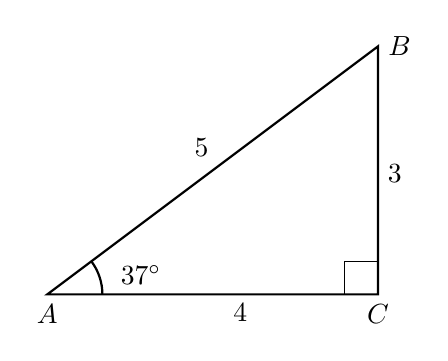
\begin{tikzpicture}[scale=0.7]
      \draw [thick]
        (0,0)node[below]{$A$}--
        (6,0)node[below]{$C$}--
        (6,4.5)node[right]{$B$}--cycle;
      \draw (6,0)++(-0.6,0)--++(0,0.6)--+(0.6,0);
      \node at (2.8,3)[below]{$5$};
      \node at (3.5,0)[below]{$4$};
      \node at (6,2.2)[right]{$3$};
      \draw [thick, -] (1,0) arc [start angle=0, end angle=37, radius=1];
      \node at (1.7,0)[above]{$37^\circ$};
    \end{tikzpicture}
  \end{flushright}

\item Find the area of the given triangle.
\begin{flushleft}
  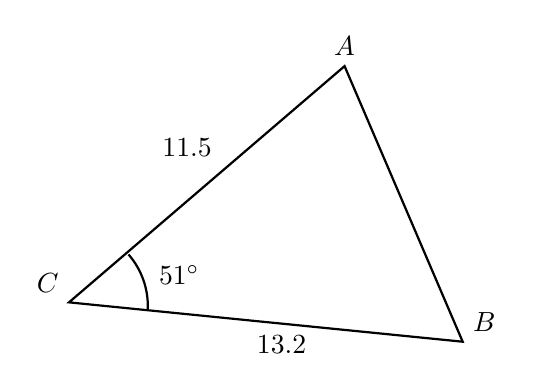
\begin{tikzpicture}[scale=1.]
    \draw [thick]
      (0,0)node[above left]{$C$}--
      (5,-0.5)node[above right]{$B$}--
      (3.5,3)node[above]{$A$}--cycle;
   \draw [thick, -] (1,-0.1) arc [start angle=-3, end angle=41, radius=1];
   \node at (1.4,0.1)[above]{$51^\circ$};
   \node at (1.5,2.2)[below]{$11.5$};
   \node at (2.7,-0.3)[below]{$13.2$};
  \end{tikzpicture}
\end{flushleft}

\item 
\begin{multicols*}{2}
\begin{enumerate}
  \item Substitute given values into the Sine rule. \vspace{1cm}
  \item Solve for the missing length $a$.
  \end{enumerate} \vspace{3cm}
\begin{flushright}
  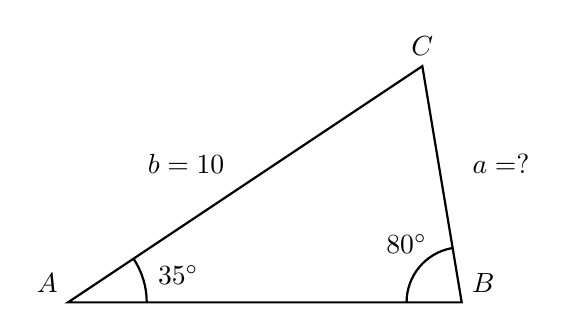
\begin{tikzpicture}[scale=1.]
    \draw [thick]
      (0,0)node[above left]{$A$}--
      (5,0)node[above right]{$B$}--
      (4.5,3)node[above]{$C$}--cycle;
   \draw [thick, -] (1,0) arc [start angle=0, end angle=34, radius=1];
   \node at (1.4,0.1)[above]{$35^\circ$};
   \draw [thick, -] (4.3,0) arc [start angle=180, end angle=100, radius=0.7];
   \node at (4.3,0.5)[above]{$80^\circ$};
   \node at (1.5,2)[below]{$b=10$};
   \node at (5.5,2)[below]{$a=?$};
  \end{tikzpicture}
\end{flushright}
\end{multicols*} \vspace{1cm}

\newpage
\item The following diagram shows triangle $ABC$, with $A\hat{B}C=60^\circ$, $A\hat{C}B=25^\circ$, and $AC=8$ cm. \\[0.25cm]
Find $AB$. \hfill \emph{diagram not to scale}
  \begin{flushright}
    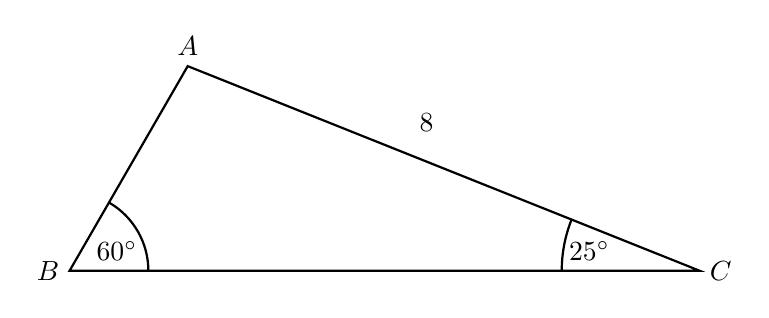
\begin{tikzpicture}[scale=1]
      \draw [thick](60:3)node[above]{$A$}--
      (0,0)node[left]{$B$}--
      (0:8)node[right]{$C$}--cycle;
      \node at (25:5)[below]{$8$};
      \draw [thick, -] (0:1) arc [start angle=0, end angle=60, radius=1];
      \node at (0:0.6)[above]{$60^\circ$};
      \draw [thick, -] (0:6.25) arc [start angle=180, end angle=158, radius=1.75];
      \node at (0:6.6)[above]{$25^\circ$};
    \end{tikzpicture}
  \end{flushright}\vspace{1cm}

\item As shown in the diagram, triangle $ABC$ has $A\hat{B}C=29^\circ$, $AB=14.1$, and $BC=16.0$. \\[0.25cm]
Find the area of the triangle. \hfill \emph{diagram not to scale}
  \begin{flushright}
    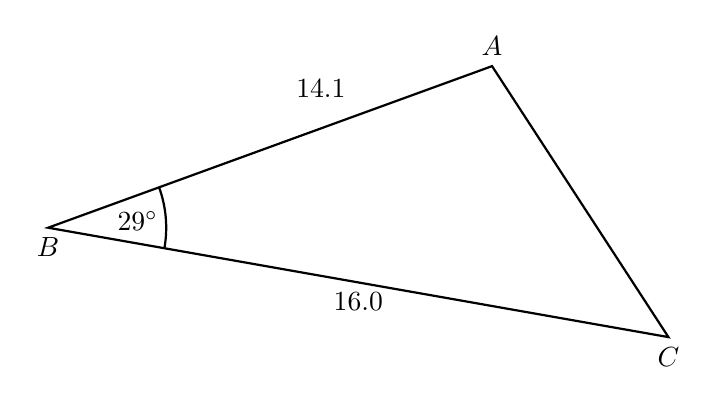
\begin{tikzpicture}[scale=1, rotate=-10]
      \draw [thick](30:6)node[above]{$A$}--
      (0,0)node[below]{$B$}--
      (0:8)node[below]{$C$}--cycle;
      \node at (40:4)[below]{$14.1$};
      \node at (0:4)[below]{$16.0$};
      \draw [thick, -] (0:1.5) arc [start angle=0, end angle=30, radius=1.5];
      \node at (2:1.15)[above]{$29^\circ$};
    \end{tikzpicture}
  \end{flushright}\vspace{1cm}

\item The following diagram shows triangle $ABC$, with $A\hat{B}C=48^\circ$, $A\hat{C}B=37^\circ$, and $AB=11.5$ cm. \\[0.25cm]
Find $AC$. \hfill \emph{diagram not to scale}
  \begin{flushright}
    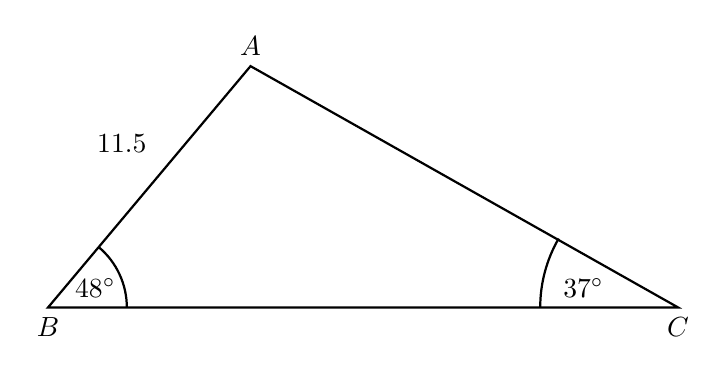
\begin{tikzpicture}[scale=1]
      \draw [thick](50:4)node[above]{$A$}--
      (0,0)node[below]{$B$}--
      (0:8)node[below]{$C$}--cycle;
      \node at (68:2.5)[below]{$11.5$};
      \draw [thick, -] (0:1) arc [start angle=0, end angle=50, radius=1];
      \node at (0:0.6)[above]{$48^\circ$};
      \draw [thick, -] (0:6.25) arc [start angle=180, end angle=150, radius=1.75];
      \node at (0:6.8)[above]{$37^\circ$};
    \end{tikzpicture}
  \end{flushright}\vspace{2cm}



\end{enumerate}
\end{document}
  